\documentclass{article}
\usepackage{graphicx} % Required for inserting images
\usepackage{float}
\usepackage{listings}
\usepackage{amssymb}
\usepackage{amsmath}
\usepackage{color}
\usepackage[margin=1in]{geometry}
\usepackage{xcolor}
\usepackage{matlab-prettifier} 
\lstset{style=Matlab-editor}




\title{MATH 543 - HW 3}
\author{Parham Khodadi}
\date{February 19, 2026}

\begin{document}

\maketitle

\section{Problem statement}
Implement the reduced QR-factorization by Classical Gram-Schmidt.

\subsection{Write a function.}
Given $A \in \mathbb{C}^{m \times n}$ the function computes $Q \in \mathbb{C}^{m \times n}$, and $R \in \mathbb{C}^{n \times n}$.
\subsection{Validate your function.}
Test that:
\begin{itemize}
    \item (i) $||A-QR|| \approx 0$
    \item (ii) $Q$ is unitary, meaning $Q^T Q = I$
    \item (iii) $R$ is upper triangular
\end{itemize}
Show 3 test cases for ($3\times3$), ($5 \times5$), and ($251\times251$) matrices.

\subsection{Compare the result.}
Look closer the the results for the ($3\times3$) and ($5 \times5$) cases and compare with the built-in (“library”) version of the QR-factorization; comment on the similarities/differences.

\subsection{Can you find a non-zero matrix where your QR-factorization breaks?}

\section{Answer and Output}
\section{Code and Output.}
My MATLAB code is found in Section \ref{MATLAB}. Its output is as follows:
\begin{verbatim}
------ Test size: 3 x 3 ------
||A - Q*R||_F      = 0.0000e+00
||Q'*Q - I||_F     = 1.0969e-15
||tril(R,-1)||_F   = 0.0000e+00
--- MATLAB qr(A,0) ---
||A - Qm*Rm||_F                        = 4.338e-16
Sign-insensitive ||abs(Q)-abs(Qm)||_F  = 7.156e-16
Sign-insensitive ||abs(R)-abs(Rm)||_F  = 6.866e-16

------ Test size: 5 x 5 ------
||A - Q*R||_F      = 1.5701e-16
||Q'*Q - I||_F     = 6.8922e-15
||tril(R,-1)||_F   = 0.0000e+00
--- MATLAB qr(A,0) ---
||A - Qm*Rm||_F                        = 1.070e-15
Sign-insensitive ||abs(Q)-abs(Qm)||_F  = 4.666e-15
Sign-insensitive ||abs(R)-abs(Rm)||_F  = 1.727e-15

------ Test size: 251 x 251 ------
||A - Q*R||_F      = 7.4948e-14
||Q'*Q - I||_F     = 1.3194e-11
||tril(R,-1)||_F   = 0.0000e+00

------ Part 4: CGS break example (Hilbert matrix) ------
||A - Q*R||_F  = 1.300e-16
||Q'*Q - I||_F = 4.515e+00
\end{verbatim}

\subsection{Why I wrote the function the way I did.}
I simply wrote the Classical Gram-Schmidt algorithm in MATLAB exactly as written on slide 23 of Lecture Notes \#6.
The only difference was that I had to account for the possibility of dividing by zero if $R_{kk} = 0$ by manually setting those points in $Q_{ik}$ to $0$.

\subsection{Result Analysis.}
\subsubsection{Part 2.}
As you can see in the output, the validity of test cases was done using the Frobenius norm. I chose to do this because a simple google search will tell you that if you stack a matrix into one long vector, the Frobenius norm is exactly the Euclidean norm of that vector:
\[||E||_F=\sqrt{\sum_{i,j}|e_{ij}|^2}\]

For each test criteria:
\begin{itemize}
    \item (i) $||A-QR|| \approx 0$ became progressively worse as the size $n$ increased.
    \item (ii) Orthogonality $Q^T Q = I$ also worsened with increasing size $n$, although still very small and close to zero.
    \item (iii) $R$'s upper triangular status consistently remained true across all three cases.
\end{itemize}

\subsubsection{Part 3.}
When comparing test cases ($3\times3$) and ($5 \times5$) in CGS and in the built-in MATLAB-library algorithm, it appears that CGS very slightly outperforms. However, the difference is increasibly subtle, on the order of $10^{-15}$ and $10^{-16}$, meaning that the difference is neglibile.

\subsubsection{Part 4.}
As you can see, I used a Hilbert matrix to push Classical Gram-Schmidt to its limit. I asked ChatGPT, "What is a type of matrix in the MATLAB library that would quickly make Classical Gram-Schmidt lose orthogonality." You can see its response in Figure \ref{fig:ChatGPT}. ChatGPT was correct, as a ($12\times12$) Hilbert matrix quickly lost orthogonality.

\section{Conclusion}
For random matrices, Classical Gram-Schmidt produces a small residual $||A-QR||$ and nearly orthonormal $Q$. For an ill-conditioned matrix, such as a Hilbert matrix, Classical Gram-Schmidt suffers loss of orthogonality due to large $||Q^TQ-I||$, illustrating the known numerical instability of Classical Gram-Schmidt due to roundoff errors.


\section{Appendix}

\subsection{MATLAB code}
\label{MATLAB}
\lstinputlisting[
  frame=single,
  numbers=left,
  caption={My MATLAB Code}
]{HW3.m}

\subsection{ChatGPT Question}
\begin{figure}[H]
    \centering
    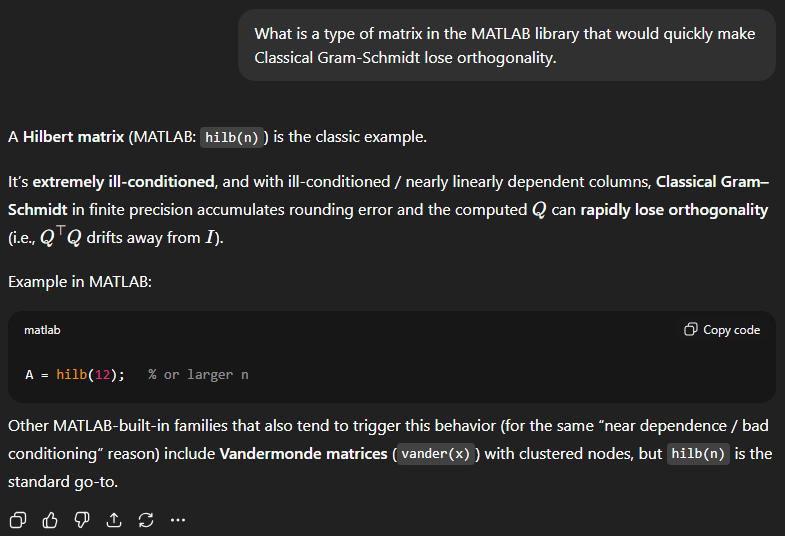
\includegraphics[width=1\linewidth]{ChatGPT_Question.png}
    \caption{Asked ChatGPT: "What is a type of matrix in the MATLAB library that would quickly make Classical Gram-Schmidt lose orthogonality."}
    \label{fig:ChatGPT}
\end{figure}


\end{document}
